\documentclass{article}

\usepackage{graphicx}
\usepackage{apacite}
\usepackage{fancyhdr}

\title{Desarrollo de aplicacion web con integracion de sistema de control versiones
  y librerias de edicion musical, para la creacion de pistas musicales de forma
  grupal}
\date{2015-07-01}
\author{Jos\'e A\~nasco}

\pagestyle{fancy}

\begin{document}
  \pagenumbering{gobble}
  \maketitle

  \newpage
  \thispagestyle{empty}
  \tableofcontents

  \newpage
  \pagenumbering{arabic}

  \section{Seccion}

  Hola mundo!

  \subsection{Subseccion}

  sub seccion de hola mundo

  \subsubsection{Subseccion}

  sub sub sub

  \paragraph{Parrafo}

  mi parrafo
  \cite{LIBROBENITO1} ha sido citado aqu\'i

  \subparagraph{Subparrafo}

  mi subparrafo

    \begin{figure}[!h]
      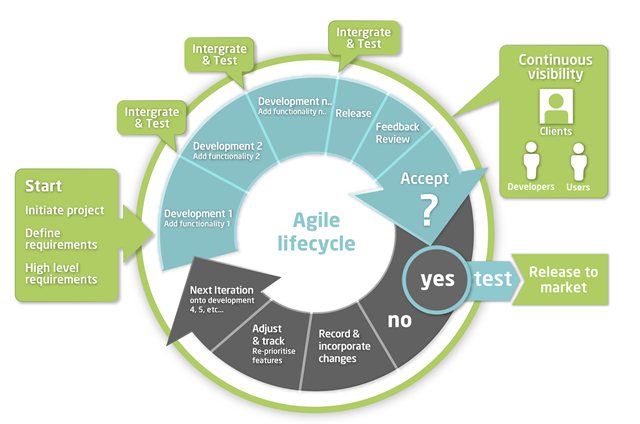
\includegraphics[width=\linewidth]{agile.png}
      \caption{Proceso Agile.}
      \label{fig:agile1}
    \end{figure}

    Figure \ref{fig:agile1} Proceso completo de Agile

  \newpage
  \section{Otra Seccion}


  \newpage
  \begin{appendix}
    \listoffigures
    \bibliographystyle{apacite}
    \bibliography{referencias}
  \end{appendix}

\end{document}
